\section{Main Result}
The chapter reports the contribution of your work.  For example, it could contain the following sub-sections to summarise the contribution of the project: Theoretical Development, Analysis and Design, Implementation and Experimental Work, Results, Observation and Discussion.

\subsection{Maths}
\begin{equation}\label{eq:BS}
\frac{\D S_t}{S_t} = r \D t + \sigma \D W_t,
\qquad S_0>0,
\end{equation}

The equation $\sigma = m a$ follows easily~\cite{Doe11}.


\subsection{Glossary and acronyms}

\Glspl{Linux} and other Unix operating systems are better then Windows because they support \gls{lvm} out of the box~\cite{Joh11}\insertref{A ref is missing here}. 

\subsection{Figures}
Here is an example~\cite{JohSil05} of how to inserta picture:

\begin{figure}[!ht]
\centering
\subfigure{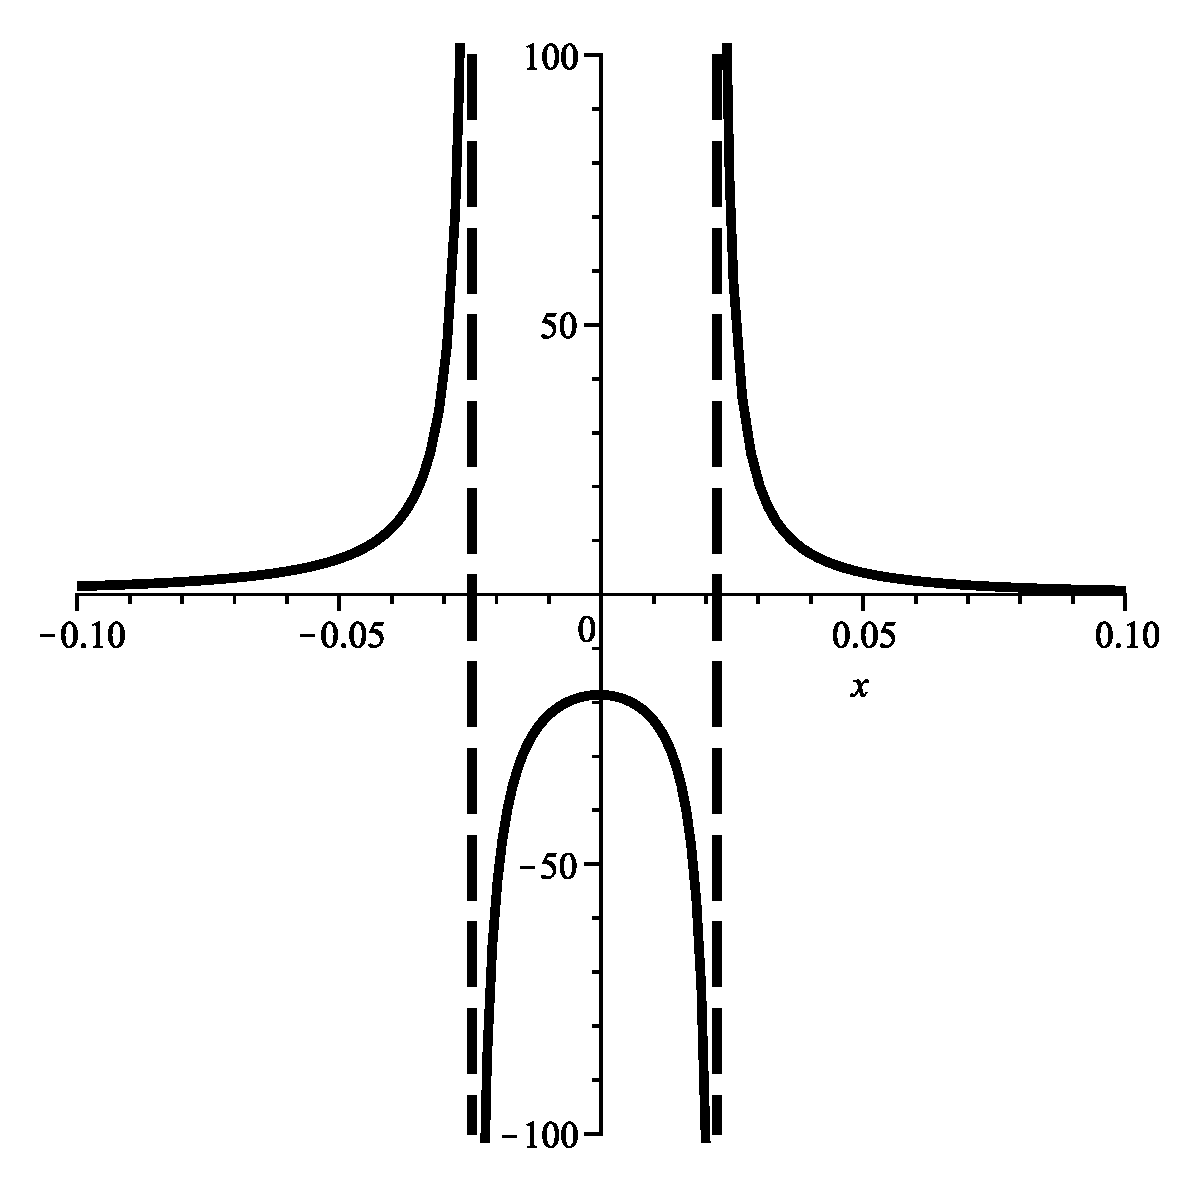
\includegraphics[scale=0.2]{figures/Picture.eps}}
\caption{This is the caption for the figure.}
\label{fig:Pict}
\end{figure}


\begin{figure}[!ht]
\centering
\missingfigure{If you know there will be a figure, but you still need to create it.}
\caption{This is the caption for the figure which is not even present.}
\label{fig:PictMis}
\end{figure}


Lorem ipsum dolor sit amet, consetetur sadipscing elitr, sed diam nonumy eirmod tempor invidunt ut labore et dolore magna aliquyam erat, sed diam voluptua. At vero eos et accusam et justo duo dolores et ea rebum. Stet clita kasd gubergren, no sea takimata sanctus est Lorem ipsum dolor sit amet. Lorem ipsum dolor sit amet, consetetur sadipscing elitr, sed diam nonumy eirmod tempor invidunt ut labore et dolore magna aliquyam erat, sed diam voluptua. At vero eos et accusam et justo duo dolores et ea rebum. Stet clita kasd gubergren, no sea takimata sanctus est Lorem ipsum dolor sit amet.\todo{This is a small Todo, please take care!}

or two side-by-side pictures:

\begin{figure}[!ht]
\centering
\subfigure{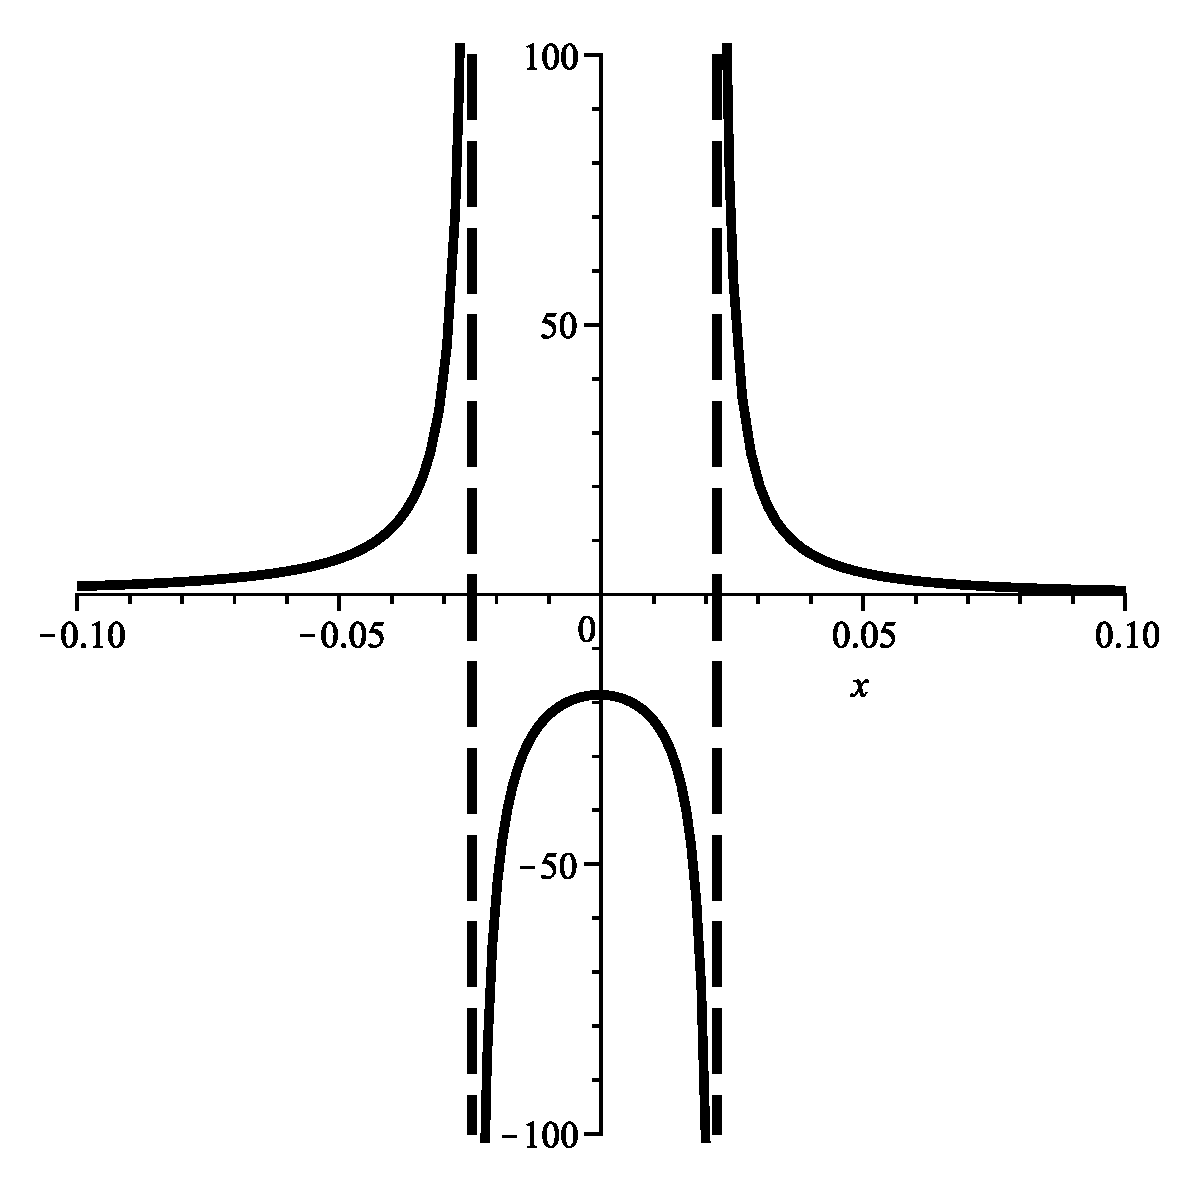
\includegraphics[scale=0.3]{figures/Picture.eps}}
\hspace{15pt}
\subfigure{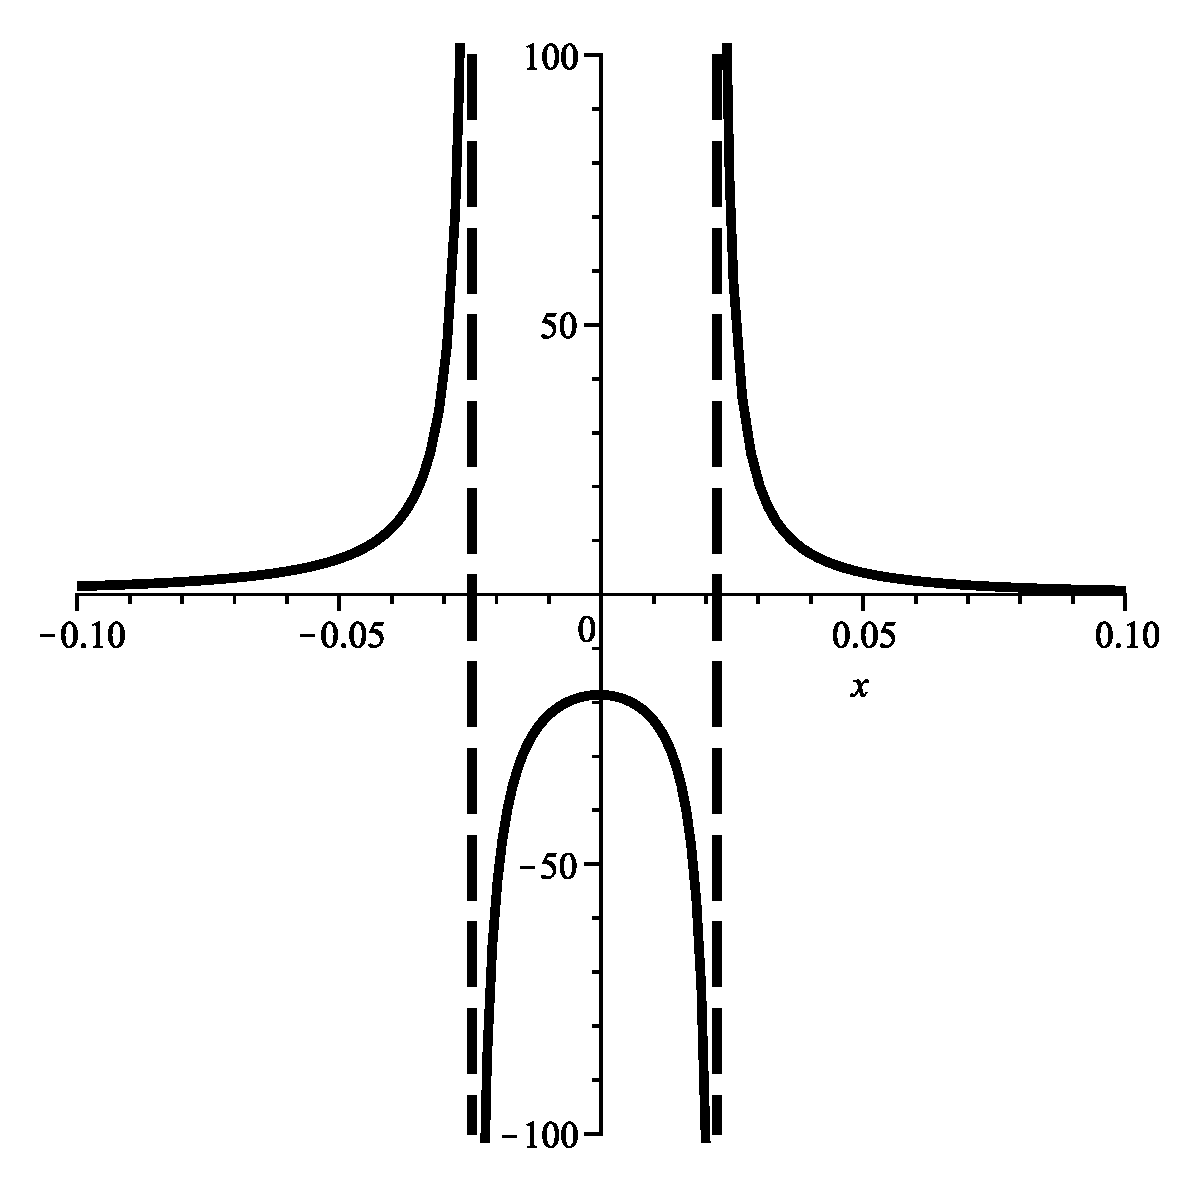
\includegraphics[scale=0.3]{figures/Picture.eps}}

\caption{Another caption}
\label{fig:Pict2}
\end{figure}



\subsection{Table}
Lorem ipsum dolor sit amet, consetetur sadipscing elitr, sed diam nonumy eirmod tempor invidunt ut labore et dolore magna aliquyam erat, sed diam voluptua. At vero eos et accusam et justo duo dolores et ea rebum. Stet clita kasd gubergren, no sea takimata sanctus est Lorem ipsum dolor sit amet. Lorem ipsum dolor sit amet, consetetur sadipscing elitr, sed diam nonumy eirmod tempor invidunt ut labore et dolore magna aliquyam erat, sed diam voluptua. At vero eos et accusam et justo duo dolores et ea rebum. Stet clita kasd gubergren, no sea takimata sanctus est Lorem ipsum dolor sit amet\explainindetail{This needs further explanation}.
\begin{table}[!ht]
	\centering
	\begin{tabular}{|l|rl|}
		\hline
		Something & Someother & Thing \\
  		Seems & to be & good\\
  		\hline
  	\end{tabular}
  	\caption{Random data for a table.}
\end{table}

Lorem ipsum dolor sit amet, consetetur sadipscing elitr, sed diam nonumy eirmod tempor invidunt ut labore et dolore magna aliquyam erat, sed diam voluptua. At vero eos et accusam et justo duo dolores et ea rebum. Stet clita kasd gubergren, no sea takimata sanctus est Lorem ipsum dolor sit amet. Lorem ipsum dolor sit amet, consetetur sadipscing elitr, sed diam nonumy eirmod tempor invidunt ut labore et dolore magna aliquyam erat, sed diam voluptua. At vero eos et accusam et justo duo dolores et ea rebum. Stet clita kasd gubergren, no sea takimata sanctus est Lorem ipsum dolor sit amet.


\section{Model calibration}
\subsection{What is calibration?}
Here is an example of a matrix\cite{website:fermentas-lambda} in $A\in\mathcal{M}_n(\RR)$:
$$
A = 
\begin{pmatrix}
a_{11} & a_{12} & \ldots & a_{1n}\\
a_{21} & \ddots & \ddots  & \vdots\\
\vdots &  \ddots & \ddots  & \vdots\\
a_{n1} &  \ldots &  \ldots & a_{1n}.
\end{pmatrix}
$$

\subsection{Numerical methods for calibration}
...


